\myChapter{Service Oriented Architecture}\label{chap:soa}
\minitoc\mtcskip
\vfill
\lettrine{P}{revious} chapter has explained some lacks in the development of EAs, mainly related with the integration of different frameworks, distributed programming and heterogeneity of computational environments, among others. This chapter explains the concept Service Oriented Architecture (SOA), with several associated technologies and methodologies, as a possible solution for these issues.

Research in Service Oriented Architectures (SOA) \citep{Papazoglou2007SOA} is an emerging field, as can be seen in Figure \ref{fig:soapapers}, obtained from the search terms {\em ``service oriented OR service-oriented''} in the Scopus \footnote{\url{http://www.scopus.com}} database. Each year more papers about the area are published. This area seeks to promote services usage and adoption, and to improve the way to use them. For example, solving a problem combining existing services in an automatic way \citep{Moussa2010ServiceComposition}.





\begin{SCfigure}[20][htb]
\centering
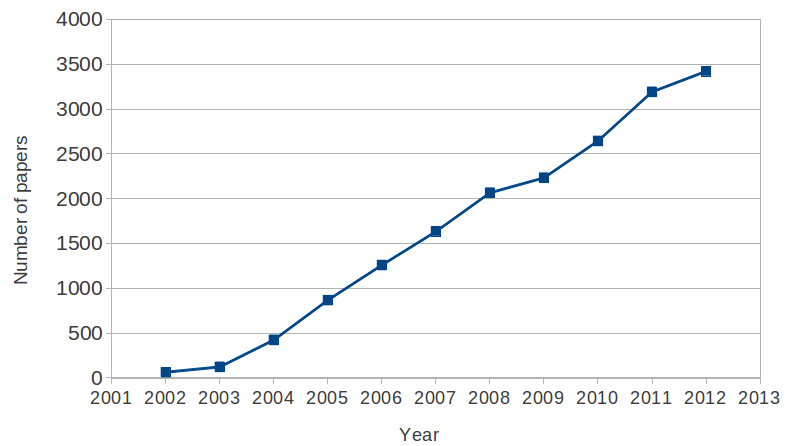
\includegraphics[width=26pc]{gfx/soa/papersYear.jpg}
\caption{Number of published papers (per year) about SOA (obtained from Scopus database).}
\label{fig:soapapers}
\end{SCfigure}


Service Oriented Architecture (SOA) is a computational
paradigm where the users interact with each other using the concept of
{\em service}. A service is a distributed entity (such as node, program,
function), used to obtain a result, increasing the integration of heterogeneous
systems (several operating systems, protocols or languages) due to
this multi-platform nature. The service users do not need to know
the language used to implement the service, and they are not
forced to use a specific technology to access that service. For
example, an evolutionary algorithms researcher could have access to a
fitness function made publicly available by another researcher at the
other side of the world without even knowing which programming language
has been used to implement it.

Also, with the advancement of the Internet, new scientific communities, based on interoperable and distributed platforms are emerging. These communities allow scientist to collaborate in their research, sharing data and remote access to their programs. To achieve this, they use SOA, obtaining the benefices of the standards it offers. Users publish and use flexible, interoperable and configurable services. These services can be created from scratch or by leveraging existing software. 

\person{Foster} \cite{Foster2005Science} defines the term ``Service Oriented
Science'' as the pursuit of scientific research using distributed and
interoperable networks, being the uniformity of
these interfaces the key to success. Thanks to it, researchers can discover and access
the services without developing specific access for each data source, or
program. Therefore, this paradigm has the potential to increase the
scientific productivity due to these public and distributed services, and also to increase the data analysis automation in computing. There are many examples that attempt to boost this paradigm, like Open Science Grid \citep{Altunay2011OpenScience} and GLOBUS \citep{Foster2005Globus}. These projects are scientific communities and globally distributed infrastructures that support scientific and integrated applications of different domains.
It is necessary to remark that services implementation technology is not the
great challenge in SOA, but to increase the effort to migrate the
existing work and to change the mind of researchers and
practitioners. 

\section{What is a Service?}

\lettrine{A}{} service can be seen as a function call which can be executed locally or remotely, and which is independent of the programming language or running platform. Services have well defined interfaces, which depends of the desired technology to implement SOA. That means that the service users do not need to know the language implementation of the service or the operating system, and they are not forced to use a specific technology to access to that service.

\begin{SCfigure}[20][htb]
\centering
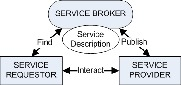
\includegraphics[width=20pc]{gfx/soa/soaDiagram.jpg}
\caption{Service interaction schema. The service provider publishes a service description that is used by the consumer to find and use the service.}
\label{fig:soadiagram}
\end{SCfigure}




Figure \ref{fig:soadiagram} shows the basic interaction among
services. First, the {\em service provider} exposes the service, publishing
its interface in the {\em service broker}. The {\em service consumer} (or
{\em requestor}) finds in the broker a service to be used and receives its
interface. Then the request is performed by the {\em consumer} (which uses or
consumes the service).  

According to \person{Channabasavaiah \etal} \cite{Channabasavaiah2003migrating} services must follow the next characteristics:

\begin{itemize}
\item All functions in SOA are services. This means that every component in SOA must be modelled as a service, or as aggregation of services. 
\item Services are autonomous. Consumers do not need to know how the service implementation performs their function., as services behave as a ``black box''.
\item Interfaces are invocable. This means that services must be undistinguishable of being local or remote, being independent of the protocol to stablish the connection.
\end{itemize}

Moreover, several implementations of a specific service  can exist (in one or several machines). The broker can choose which one to use  each time, or offer another if a service is unavailable. Implementations  may also have a different behaviour, so the researcher can take advantage to create an auto-adaptive algorithm to select different implementations according to some criteria. Figure \ref{fig:servicebasic} shows this special interaction, where two different implementations of an operator interface exist (even using different languages) and the broker has chosen one of them.


The service broker in a SOA can be implemented in several ways and have
different behaviors: for example, the implementations of the services to be used can be
defined in a text file (if the services do not change in execution
time). However, the broker can also assign implementations to
interfaces in an automatic way, or using several rules, for example, in the context of EAs,
to distribute a fitness between several machines activated while the
algorithm is running. 


\begin{SCfigure}[20][htb]
\centering
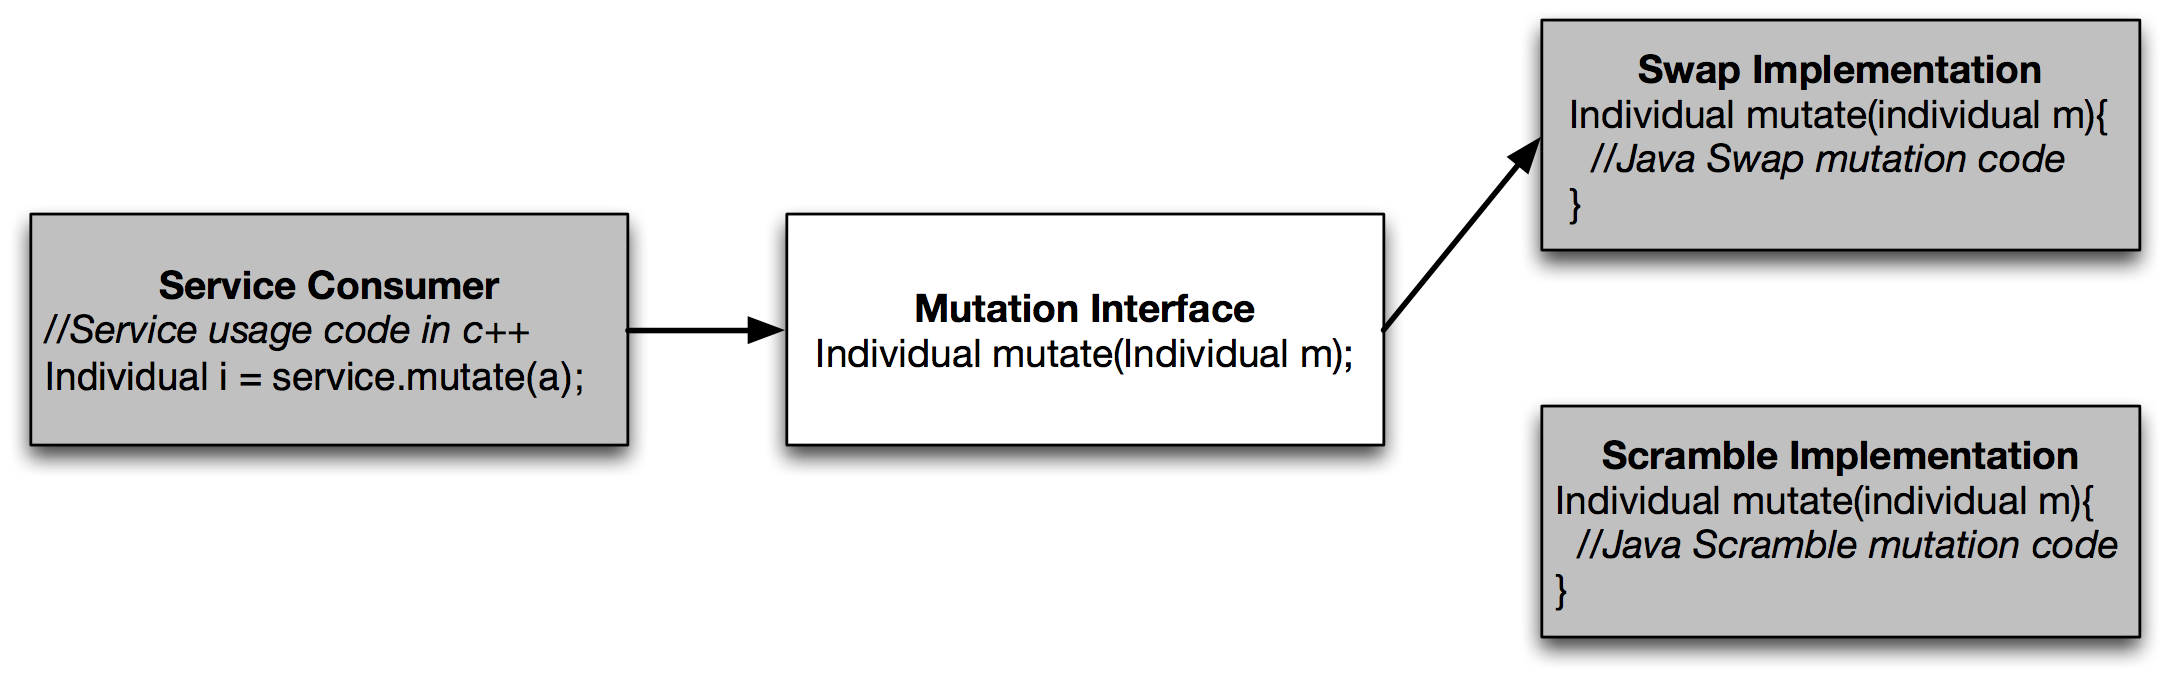
\includegraphics[width=26pc]{gfx/soa/exampleSOA.jpg}
\caption{Example of usage of a service implementation.}
\label{fig:servicebasic}
\end{SCfigure}




An important SOA capability is that it is not focused on a specific
implementation, but offers a set of guidelines to help the
developers. In \citep{Arsanjani2008SOMA} these guidelines and good practices, and also the differences between SOA and Object Oriented
Programming (OOP) are
explained: the main difference between SOA and imperative programming or OOP is the order of service execution. This order is not necessarily static, because the services are designed to be used in a non-established and configurable order. Furthermore, another important difference is that services can be dynamically discovered and used (while in OOP must be previously known and can not change during execution), being also one of the most important capabilities the (optional) distribution in a network. Finally, in OOP the programming language must be the same for each method call.

\section{Implementation technologies}

\lettrine{D}{espite} the fact the concept service is independent to the technology used, there exist several ways to use and implement them, being the most extended the Web Services, \definicion{ebXML}{Electronic Business XML} and \definicion{Open Service Gateway Initiative}{OSGi}.

\subsection{Web Services}

One of most popular services implementations are the Web Services \cite{Papazoglou2007SOA}. A web service is a service that is available over Internet that uses any standardized XML (eXtended Meta Language) \cite{XML} messaging system, and it is not tied to any specific language or operating system \cite{Cerami2002Webservices}.  As SOA proposes, web services should be self-describing (using a standardized grammar) and self-discoverable.

\subsubsection{Messaging system} There are several alternatives to the messaging system, for example, using SOAP or XML-RPC. SOAP (Simple Object Access Protocol) is a standard protocol proposed by the W3C \cite{SOAP} to interface web  which  extends the XML remote procedure call (XML-RPC) standard. 
SOAP is a complete and mature protocol that allows to perform remote method calls to distributed routines (services) based on an XML interface.

SOAP clients can access to objects and methods that are residing in remote servers, using a standard mechanism that makes transparent the details of implementation, such us the programming language of the
routines, the operating system or the platform used by the provider of the service. 
At the moment, there exist complete implementations of SOAP for Perl, Java, Python, C++ and most modern languages.
In opposite to other remote procedure call methods, such as RMI (\emph{remote method invocation}, used by the Java language) or XML-RPC, SOAP has two main advantages: it can be used with any programming language, and it can use any type of transport (\definicion{HTTP}{HyperText Transfer Protocol}, \definicion{SHTTP}{Secure HTTP}, \definicion{TCP}{Transmission Control Protocol}, \definicion{SMTP}{Simple Mail Transfer Protocol}, \definicion{POP}{Post Office Protocol} and other protocols). In this way, SOAP constitutes a high level protocol, making easy the task of distributing objects among different servers, and avoiding the difficulties derived of defining the message formats, nor the explicit call to remote servers.


\subsubsection{Self-description} The interfaces of the methods that can be accessed are specified by a Web Services Description Language (WSDL) \cite{WSDL}. The WSDL of a web service consists in an XML description of its interface, i.e., it is a file that describes the name of the methods, the parameters (number and type) and the type of response.

\subsubsection{Self-discovery} UDDI ({\em Universal Description, Discovery and Integration}) \cite{UDDI} is a technical specification for describing, discovering and integrating web services \cite{Cerami2002Webservices}. This specification includes APIs for the storage and retrieval of information (also in an standardized XML format).


\subsubsection{Other standardizations} One of the advantages of using web services, is that the application stack is growing with the WS-Extensions. That is, the basic specifications of Web Services (such as SOAP) can be extended with transactions, security or messaging, for example. The most used are \cite{Papazoglou2007SOA}:
\begin{itemize}
  \item WS-Adressing  (authentication)
  \item WS-Security , WS-SecureConversation  and WS-Trust  (authorization and secure messaging)
  \item WS-Policy and WS-Metadata Exchange (policy mechanisms for interactions)
  \item WS-Reliable Messaging  and WS-Transaction (add-on mechanisms for the communication channel)
\end{itemize}

Also, functional extensions, such as WSRF \cite{WSRF}, allows the discovery, inspection and interaction with stateful resources in standard and interoperable ways. Finally, BPEL ({\em Business Process Execution Language})  \cite{BPEL} is an XML-based language to control the invocation of different Web services with added business logic to help large-scale programming.

Several studies about e-science taking advantage of web services can be found in bibliography \cite{Oinn04Taverna,davidson08workflows,Ludascher06Kepler,Perera06workflows}.

\subsection{REST}
Representational State Transfer (REST)\footnote{\url{http://en.wikipedia.org/wiki/Representational_state_transfer}} is an alternative method for building web services.
This technology was proposed and defined by \person{Fielding} in \cite{Fielding2002}.

In a REST-style architecture, a client sends requests to the server who process them and return responses to the client.
Requests and responses represent resources that can be addressed by an Uniform resource identifier (URI). Usually, resources are documents or programs the client need to access to.

REST usually works on the HTTP protocol, however it can be based on other protocols that provide the appropriate mechanisms to send requests and return responses.

In a REST environment, while servers are not concerned with the client state, clients only take care about their own state and how to address resources on the server using URIs. Moreover, clients can cache responses to improve performance.
As the client-server communication is stateless, servers are simpler and more scalable. 
Taking this into account, if the REST interface is not altered, servers and clients can be modified independently.
Finally, servers can customize the functionality of the clients by sending logic (code) to them that can be executed.


REST web services are simple and lightweight (as no extra XML markup is needed), their message format is readable by humans, they are easy to build, and finally, developments achieve a high performance \cite{Daigneau2011}. The main differentiating factor is that Web Services using SOAP tend to be operation-based, while REST services are resource-based.

\subsection{ebXML}
ebXML defines a set of standards that allows the enterprises negotiate their products through the Internet. It is based on a well-defined documents interchange using a contract-based approach \cite{Patil03ebxmlVsWS}, providing a specification for messaging, registry/repositories and business processes description, and unlike other approaches, it is an horizontal standard (it is not oriented towards a specific industry sector). On the contrary, Web Services expose any kind of applications to the Web, so anyone can call them (service approach). Another main difference between Web Services and ebXML is that the former is based on BPEL, which can only describe the scenario inside a company, due to it has not all the information of the services being orchestrated, while the latter can be used to model a global choreography among several companies. Due to this, and because it is mainly focused to commercial and business processes we are not going to delve into this technology in this thesis.

\subsection{OSGi}

OSGi, was proposed by a consortium of more than
eighty companies in order to develop an infrastructure for the
deployment of service in heterogeneous network of devices, mainly
oriented to domotics \cite{GarciaSanchez2013Gateway}. Nowadays it defines a
specification for a Service Oriented Architecture for virtual
machines (VMs). It provides very desirables features, like
packet abstraction, life-cycle management, packaging or versioning,
allowing significant reduction of the building, support and deployment
complexity of the applications. 

OSGi technology allows dynamic discovery of new components, to increase the collaboration and to minimize and manage the coupling
among modules. Moreover, the
OSGi Alliance has developed several standard component interfaces for
common usage patterns, like HTTP servers, configuration, logs, security,
management or XML management among others, whose implementations can
be obtained by third-parties. Nowadays there are some challenges 
in the OSGi development \cite{Kriens2008OsgiChallenges}, but they only affect the creation of very complex applications.

This advantages are not so
                               costly, as can be thought: the OSGi
                                framework can be implemented in a
                                {\em jar} file\footnote{A jar file is
                                a file that groups the compiled Java
                                files.} of 300KB. Also, and different
                                of the normal usage of Java, each
                                class pre-charges only the other
                                classes to use, not all. Also is
                                non-intrusive: the code to be
                                executed in OSGi can be executed
                                without it. Finally, from its
                                specification in 1998 has been widely
                                used as base in big projects: the
                                Eclipse \definicion{IDE}{Integrated Development
                                Environment} is built over OSGi, and
                                also big application servers
                               (Glassfish\footnote{\url{http://glassfish.java.net}} 
                               or IBM Websphere \footnote{\url{http://www.ibm.com/software/websphere/}}) or
                               residential gateways
                               \cite{GarciaSanchez2013Gateway}, among other
                               examples. 

\subsubsection{OSGi Architecture}
To understand how OSGi \cite{Moussa2010Composition} works and which capabilities could offer to the EA practitioners it is necessary to understand how OSGi is built. OSGi has a layered model that is depicted in Figure \ref{fig:osgi-original}. The terms present in this Figure are:

\begin{itemize}
\item Bundles: Bundles are the OSGi components made by developers. Is a normal {\em jar} file including Java classes and interfaces with different MANIFEST.MF and extra files (such as the Service Descriptions).
\item Services: This layer connects bundles in a dynamic way by offering a publish-find-bind model.
\item Life-Cycle: The API to install, start, stop, update, and uninstall bundles.
\item Modules: This layer defines how a bundle can import and export code (using the MANIFEST.MF file).
\item Security: Security aspects are handled in this layer.
\item Execution Environment: Defines what methods and classes are available in a specific platform. For example, mobile devices have less Java classes due to performance constraints.
\end{itemize}

\begin{SCfigure}[20][htb]
\centering
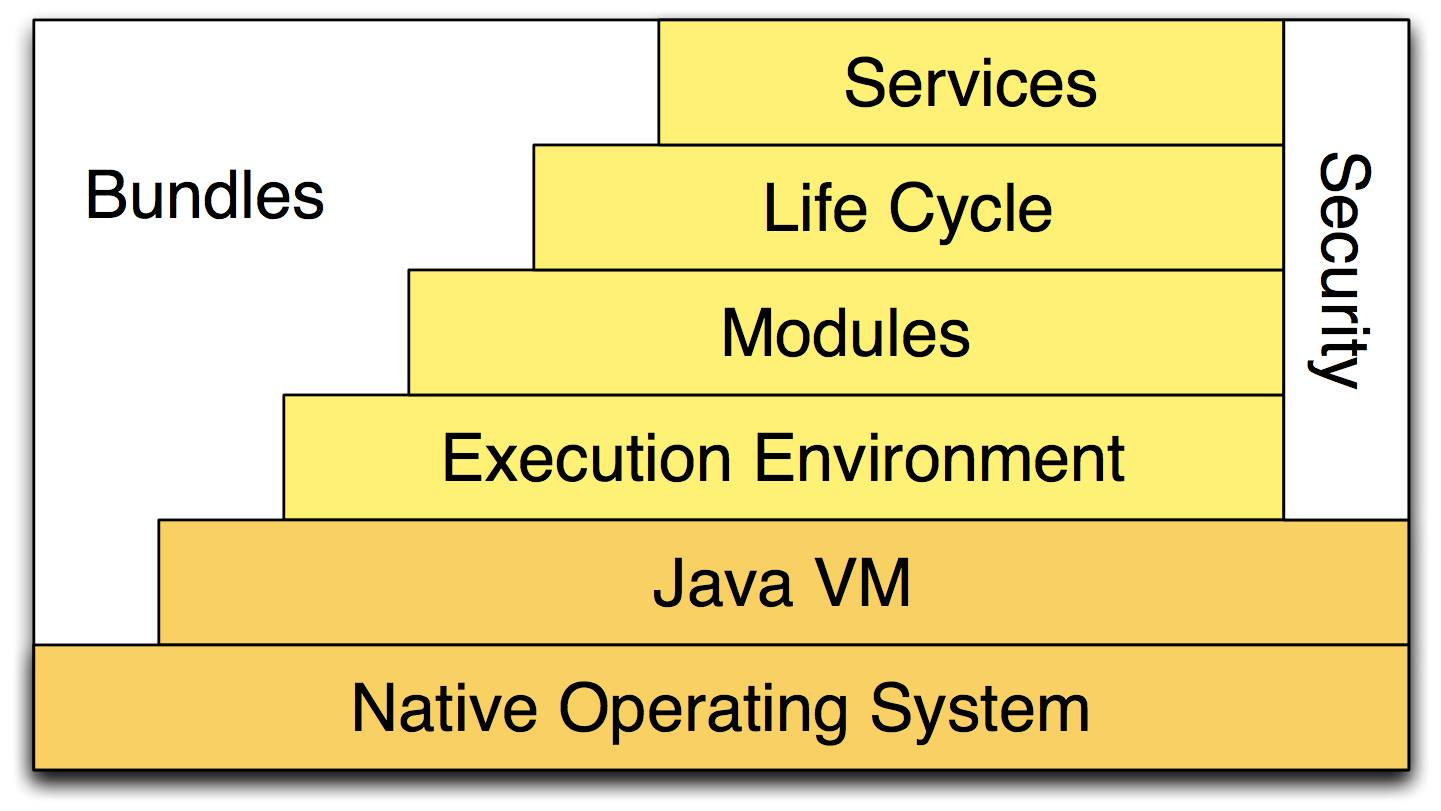
\includegraphics[width=26pc]{gfx/soa/osgi-oficial.jpg}
\caption{OSGi layered architecture. Every layer is built from the one just below.}
\label{fig:osgi-original}
\end{SCfigure}






\subsubsection{OSGi configuration files}
Regarding to explained OSGi layers how to use all OSGi capabilities is shown next. 

OSGi implements a dynamic component model, unlike normal Java
environments. Applications or components (also called
\emph{bundles}) can be remotely installed, started, stopped, updated
or uninstalled on the fly; moreover, the classes and
packaging management is specified in detail. The OSGi framework provides
APIs for the management of services that are exposed or used by the
bundles.

Java programmers are familiar with the {\em jar} concept. The first difference among a {\em bundle} and a {\em jar} is that the second has a MANIFEST.MF file adapted to be used in OSGi. This file indicates which classes imports or exports the {\em bundle}. An example can be seen in Figure \ref{fig:manifest}. This file shows the name of the bundle and its version (this is useful to select specific services), and the execution environment (that is, the Java Virtual Machine required). Also, this file specifies the XML files of the declarative services (in section {\em Service-Component}). However, this {\em bundle} can be used as a normal {\em jar} outside OSGi.

\begin{SCfigure}[20][htb]
\noindent
\ttfamily
\hlstd{}{\bf Manifest-Version:} 1.0\\
\hlstd{}{\bf Bundle-ManifestVersion:} 2\\
\hlstd{}{\bf Bundle-Name:} VRP\\
\hlstd{}{\bf Bundle-SymbolicName:} VRP\\
\hlstd{}{\bf Bundle-Version:} 1.0.0\\
\hlstd{}{\bf Bundle-RequiredExecutionEnvironment:} JAVA-1.6\\
\hlstd{}{\bf Import-Package:}  es.ugr.osgiliath,\\
 \hlstd{}  es.ugr.osgiliath.algorithms,\\
\hlstd{} es.ugr.osgiliath.events,\\
 \hlstd{}es.ugr.osgiliath.evolutionary,\\
 \hlstd{}es.ugr.osgiliath.evolutionary.basiccomponents.genomes,\\
 \hlstd{}es.ugr.osgiliath.evolutionary.basiccomponents.individuals,\\
 \hlstd{}es.ugr.osgiliath.evolutionary.elements,\\
 \hlstd{}es.ugr.osgiliath.evolutionary.individual,\\
 \hlstd{}es.ugr.osgiliath.evolutionary.migrator,\\
 \hlstd{}es.ugr.osgiliath.geneticalgorithm.distributed,\\
 \hlstd{}es.ugr.osgiliath.problem\\
\hlstd{}{\bf Export-Package:} es.ugr.osgiliath.vrp,\\
 \hlstd{}es.ugr.osgiliath.vrp.individual\\
\hlstd{}\hlkwa{Service-Component:} OSGI-INF/vrpinitializer.xml,\\
OSGI-INF/vrpfitnesscalculator.xml,\\
 OSGI-INF/vrpcrossover.xml,\\
 OSGI-INF/vrpmutation.xml\\
\mbox{}
 
\normalfont
\caption{Example of MANIFEST.MF. This example defines which packages are necessary to activate the bundle and which packages are exported.}
\label{fig:manifest}
\end {SCfigure}





In normal environments, to create a specific implementation of an interface (i.e. {\em FitnessCalculator}) is as follows:

%\begin{lstlisting}
\begin{minted}[mathescape,
               linenos,
               frame=lines,
               framesep=2mm]{java}
class EvolutionaryAlgorithm implements Algorithm{
 FitnessCalculator fc;
 //A new instance is bound to a reference
 fc = new ExampleFunction();
}
\end{minted}
%\end{lstlisting}


With Declarative Services, the {\em new ExampleFunction()} part is not used, so if a new implementation is desired no code recompilation is necessary.  Figure \ref{fig:ds} shows a declarative service description file, which establish in execution time which implementation is bound to the interfaces. This example indicates that the implementation of service {\em FitnessCalculator} is {\em VRPFitnessCalculator}, but this service is not activated until all their references (other services, like {\em TransportData}) are also activated. The tag {\em cardinality} means that at least one service of that kind must exist (the first {\em 1} represents optionality) and  the second part (the other {\em 1} indicates the number of different implementations that can be managed: one ({\em 1}) or many ({\em *}).  We need to create XML files for the rest of services to expose (i.e. {\em TransportData}). The file where these capabilities are defined is declared in section {\em Service-Component} of MANIFEST.MF file, as can be seen in Figure \ref{fig:manifest}.


%\noindent
%\ttfamily
%\hlstd{}\hlopt{$<$}\hlstd{?xml\ version}\hlopt{=}\hlstd{"}\hlnum{1.0}\hlstd{"\ encoding}\hlopt{=}\hlstd{"UTF{-}8"?}\hlopt{$>$}\hspace*{\fill}\\
%\hlstd{}\hlopt{$<$}\hlstd{scr}\hlopt{:}\hlstd{component\ xmlns}\hlopt{:}\hlstd{scr}\hlopt{=}\hlstd{"http}\hlopt{://}\hlstd{www}\hlopt{.}\hlstd{osgi}\hlopt{.}\hlstd{org}\hlopt{/}\hlstd{xmlns}\hlopt{/}\hlstd{scr}\hlopt{/}\hlstd{v1}\hlopt{.}\hlstd{1}\hlnum{.0}\hlstd{"\ name}\hlopt{=}\hlstd{"VRPFitnessCalculator"}\hlopt{$>$}\hspace*{\fill}\\
%\hlstd{}\hlstd{\ \ \ }\hlstd{}\hlopt{$<$}\hlstd{implementation\ class}\hlopt{=}\hlstd{"es}\hlopt{.}\hlstd{ugr}\hlopt{.}\hlstd{osgiliath}\hlopt{.}\hlstd{vrp}\hlopt{.}\hlstd{VRPFitnessCalculator"}\hlopt{/$>$}\hspace*{\fill}\\
%\hlstd{}\hlstd{\ \ \ }\hlstd{}\hlopt{$<$}\hlstd{service}\hlopt{$>$}\hspace*{\fill}\\
%\hlstd{}\hlstd{\ \ \ \ \ \ }\hlstd{}\hlopt{$<$}\hlstd{}\hlkwa{provide\ }\hlstd{interface}\hlopt{=}\hlstd{"es}\hlopt{.}\hlstd{ugr}\hlopt{.}\hlstd{osgiliath}\hlopt{.}\hlstd{evolutionary}\hlopt{.}\hlstd{elements}\hlopt{.}\hlstd{FitnessCalculator"}\hlopt{/$>$}\hspace*{\fill}\\
%\hlstd{}\hlstd{\ \ \ }\hlstd{}\hlopt{$<$/}\hlstd{service}\hlopt{$>$}\hspace*{\fill}\\
%\hlstd{}\hlstd{\ \ \ }\hlstd{}\hlopt{$<$}\hlstd{reference\ bind}\hlopt{=}\hlstd{"setTransportData"\ \hspace*{\fill}\\
%}\hlstd{\ \ \ \ }\hlstd{unbind}\hlopt{=}\hlstd{"unsetTransportData"\hspace*{\fill}\\
%}\hlstd{\ \ \ \ }\hlstd{cardinality}\hlopt{=}\hlstd{"}\hlnum{1}\hlstd{}\hlopt{.}\hlstd{}\hlnum{.1}\hlstd{"\ \hspace*{\fill}\\
%}\hlstd{\ \ \ \ }\hlstd{interface}\hlopt{=}\hlstd{"es}\hlopt{.}\hlstd{ugr}\hlopt{.}\hlstd{osgiliath}\hlopt{.}\hlstd{vrp}\hlopt{.}\hlstd{TransportData"\ \hspace*{\fill}\\
%}\hlstd{\ \ \ \ }\hlstd{name}\hlopt{=}\hlstd{"TransportData"\ \hspace*{\fill}\\
%}\hlstd{\ \ \ \ }\hlstd{policy}\hlopt{=}\hlstd{"static"\hspace*{\fill}\\
%}\hlstd{\ \ \ }\hlstd{}\hlopt{/$>$}\hspace*{\fill}\\
%\hlstd{}\hlstd{\ \ \ }\hlstd{}\hlopt{$<$}\hlstd{property\ name}\hlopt{=}\hlstd{"name"\ }\hlkwa{type}\hlstd{}\hlopt{=}\hlstd{"String"\ }\hlkwa{value}\hlstd{}\hlopt{=}\hlstd{"vrpfitnesscalculator"}\hlopt{/$>$}\hspace*{\fill}\\
%\hlstd{}\hlopt{$<$/}\hlstd{scr}\hlopt{:}\hlstd{component}\hlopt{$>$}\hlstd{}\hspace*{\fill}\\
%\mbox{}
%\normalfont

\begin{figure*}[t]
\begin{minted}[linenos,
               fontsize=\scriptsize,
               frame=lines,
               framesep=2mm]{xml}
<?xml version="1.0" encoding="UTF-8"?>
<scr:component xmlns:scr="http://www.osgi.org/xmlns/scr/v1.1.0"
name="VRPFitnessCalculator">
<implementation class="es.ugr.osgiliath.vrp.VRPFitnessCalculator"/>
<service>
<provide 
interface="es.ugr.osgiliath.evolutionary.elements.FitnessCalculator"/>
</service>
<reference bind="setTransportData"
unbind="unsetTransportData"
cardinality="1..1"
interface="es.ugr.osgiliath.vrp.TransportData"
name="TransportData"
policy="static"
/>
<property name="name" type="String"
value="vrpfitnesscalculator"/>
</scr:component>
\end{minted}
\caption{Service Description. This documents indicates that the implementation of the service {\em FitnessCalculator} is {\em VRPFitnessCalculator}, but it can not activate until their references (other services) are activated.}
\label{fig:ds}
\end {figure*}

 Next code shows the code for this implementation:

\begin{minted}[mathescape,
               linenos,
               frame=lines,
               framesep=2mm]{java}
class VRPFitnessCalculator implements FitnessCalculator{
 //Other service references,
 TransportData tdata;
 
 //Methods to bind/unbind each reference
 public TransportData 
    setTransportData(TransportData tdata){
  this.tdata = tdata;
 }
	
 public void 
    unsetTransportData(TransportData tdata){
  this.tdata = null;
 }

 //Implementation of the interface method
 List<Fitness> calculateFitness(List<Individual> inds){
 	...
 }
}
\end{minted}

%We have to say that in future work these kind of files will be automatically created, being this task transparent to future users of the OSGiLiatH framework.

\subsubsection{Event Administration}
The Event Administration in OSGi lets the usage of a blackboard communication architecture where bundles can broadcast or receive events without notice which bundles are sending or receiving these events.

%Acquire a reference to the EventAdmin OSGi service, it implements the org.osgi.service.event.EventAdmin.
%Pick a topic name for the event and make sure that it follows Topic Naming Conventions mentioned above.
%Fill Event Properties in a dictionary that will be passed as a parameter to the publish method.
%Having the Topic Name and Properties, ready invoke one of the following methods of the Event Admin service: postEvent or sendEvent - while postEvent initiates synchronous delivery of the event, sendEvent initiates asynchronous delivery of the event. So by default, your option should be postEvent method unless you have strict requirements to not continue execution until all handlers of the event handle it.

The steps necessary to send events to other bundles:
\begin{itemize}
\item Acquire a reference to the EventAdmin OSGi service (via Declarative Services, for example).
\item Pick a topic name for the event (for example {\em ``es/ugr/osgiliath/algorithms/endgeneration''})
\item Send the event using the {\em postEvent} method of EventAdmin, with the topic plus other desired properties %(poner lo de sincrono/asincrono?)
\end{itemize}

Code to send an event to other bundles is shown below. The programmer specifies the topic String and optional properties to send to other bundles that are listening. The {\em eventAdmin} variable is a reference to {\em ``org.osgi.service.event. EventAdmin''} service, obtained via Declarative Services or by hand (not showed).

\begin{minted}[mathescape,
               linenos,
               frame=lines,
               framesep=2mm]{java}
Properties props = new Properties(); //Optional
String topic = 
   "es/ugr/osgiliath/algorithms/endgeneration";
Event evt = new Event(topic,props);
eventAdmin.postEvent(evt);
\end{minted}
		
For the other hand, the steps to handle events are:
\begin{itemize}
\item Register a service that implements the OSGi EventHandler interface (via Declarative Services or manually).
\item Specify in this service the topics to subscribe to. For example, the String {\em ``es/ugr/osgiliath/algorithms/*''} (the * is a wildcard) inside the $<$property$>$ tag in the Service Description.
\item Overwrite the handleEvent method of this interface with the desired code.
\end{itemize}

This code shows how to handle events. In this case we have published the {\em ExampleService} with the implementation {\em ExampleImpl}, that is listening under the topic {\em ``es/ugr/osgiliath/algorithms/*''}.

\begin{minted}[mathescape,
               linenos,
               frame=lines,
               framesep=2mm]{java}
class ExampleImpl implements ExampleService,EventHandler{

 public void handleEvent(Event ev){
  if(evt.getTopic().endsWith("endgeneration")){
   // An event with topic 
   // "es/ugr/osgiliath/algorithms
   // /endgeneration"
   System.out.println("Generation over");
  else{
   // Other event with topic starts with
   // "es/ugr/osgiliath/algorithms/"
   System.out.println("Other event received");
  }
 }
}
\end{minted}


\subsubsection{Distribution}
As previously said, all services must be capable to be indistinguishable of being a local or a remote service. Services can be distributed using the OSGi features. In this case, the distribution is performed using the service descriptor to set which service is distributable and which is the distribution technology that provides service discovering and data transmission.

OSGi allows several implementations for the service distribution. ECF (Eclipse Communication Framework)\footnote{\url{http://www.eclipse.org/ecf/}} has been chosen because it is the most mature and accepted implementation \cite{petzold2011dynamic}, and it also supports the largest number of transmission protocols, including both synchronous and asynchronous communication. It provides a modular implementation of the OSGi 4.2 Remote Services standard\footnote{\url{http://www.osgi.org/Release4/Download}}. This specification uses the OSGi service registry to expose remote services to other machines (being indistinguishable from the local ones). ECF also separates the source code from the discovery and transmission mechanism, allowing users to apply the most adequate technology to their needs, and providing the integration with existing applications. % For example, the lines of Figure \ref{fig:remote} have been added to the service descriptor of {\em MOP2 Fitness Calculator} to distribute it in the local network.

ECF includes a number of protocols for service discovery and service providers:
\begin{itemize}
\item Service Discovery API: Includes protocols to announce and discover remote services: Zeroconf, SLP/RFC 2608, Zookeeper, file-based and others \footnote{\url{http://wiki.eclipse.org/ECF_API_Docs\#Discovery_API}}.
\item Remote Service API: Includes protocols to establish the communication (data streams, formats and others): R-OSGi, ActiveMQ/JMS, REST, SOAP, XMPP, ECF Generic \footnote{\url{http://wiki.eclipse.org/ECF_API_Docs\#Remote_Services_API}}. This allow to communicate to systems that do not use OSGi or Java.
\end{itemize}

\section{Methodologies for developing SOA}
Regardless of the chosen SOA framework, the business processes of the platform must be analysed and modelled. So it is necessary to use a consistent and well-defined methodology to design a model based on a machine-readable description \cite{Garcia09UMM}. {\em Business-Centric Methodology (BCM) for Enterprise Agility and Interoperability} \cite{Oasis03BCM} is a roadmap for the development and implementation of procedures to create effective, efficient, and sustainable interoperability mechanisms. It has been developed by OASIS, the same consortium that created BPEL or UDDI, among others, and it is complementary to other existent architectures and technologies designed to build business oriented services, like ebXML or Web Services. BCM is formed by a set of model layers with a step-guide process, and an information pyramid to align the semantic information of partners. This allows the participation of business experts and the creation of a very large documentation repository. Nevertheless, this methodology has some disadvantages: it has a very large learning curve and it is not very extended yet. 

{\em SOMA} (Service Oriented Modelling and Architecture) \cite{Arsanjani2008SOMA} is an architecture proposed by IBM to model service oriented processes. It lets the identification, specification and implementation of services inside the SOA paradigm. To achieve this tasks, it proposes a top-down modelling oriented to intra-enterprise services (service-oriented instead of business-oriented).

{\em \definicion{UN/CEFACTs}{United Nations Center for Trade Facilitation and Electronic Business} Modelling Methodology (UMM)} \cite{Hofreiter06UMM} is an approach to model the business services that each partner must provide in order to perform a \definicion{B2B}{Business to Business} collaboration. It has a complete meta-model about business processes and business information, including a process analysis methodology. It is interesting to show that UMM provides and supports components to capture the knowledge about the business processes, and that it is independent of the underlying implementation technology (ebXML, Web Services, \definicion{CORBA}{Common Object Request Broker Architecture} or \definicion{EDI}{Electronic data interchange}). Furthermore, because UMM extends \definicion{UML}{Universal Modelling Language}, we could say that this methodology is more easily adaptable, due to the high development, acceptance and maturity of UML \cite{Garcia09UMM}. In fact, a survey of B2B modelling languages show that UMM is the most complete approach \cite{Folmer08b2b}.

\section{Benefits of using SOA in Evolutionary Algorithms Area}

\lettrine{S}{OA} has been previously used in the EA area. For example, web services have been used in the grid area for optimization problems, as can be seen in the works of \cite{grid1,grid2,grid3,grid5}, where services are defined using WSDL interfaces and other transmission mechanisms (such as Remote Procedure Call \citep{grid6,grid7}). Although there also exist EAs to be executed in grids \citep{grid8,grid4,grid10}) no information about how to design these services for EAs has been provided in previous works. 

In the previous chapter we described several lacks in the Evolutionary Algorithms area, such as the new trends of distributed programming where nodes enter and exit in runtime, or the incompatibility between frameworks, for example. All these facts have motivated us to create a proper way to define services for evolutionary algorithms. The elements that combine an EA are candidate to be designed as services, as they can behave as input/output functions, allowing the next issues:  

\begin{itemize}
\item Services can be combined in different ways to create the different types of EAs. The services must be designed taking into account the elements that form an EA. 
\item Services are independent of the used technology or the communication protocol. For example, a fitness service can be distributed or local.
\item Services are not aware of the order of execution, so this paradigm can fit with new parallel approaches for EAs, where nodes control is not centralized. 
\item Existent EA frameworks could also be adapted to be accessed as services.
\item SOA is the key to develop Open Science \cite{Foster2005Science}.
\end{itemize}

Even as SOA is used extensively in software development area, it is not widely accepted in the main EA software. The authors should improve their frameworks adding SOA technologies in order to facilitate the communication and integration among them. Although all the approaches described in previous chapter are focused on the implementation of distributed EAs, the abstraction level of each alternative can be quite different, as shown in Figure \ref{fig:soagrid}. This figure has been updated from the one presented in \cite{SOALIB}. As SOA is a methodology and not a technology, areas such as Evolutionary Robotics, or EA classic frameworks can use SOA to be designed and developed. Implementation technologies, such as Web Services are the gap between SOA (abstract) and grid (infrastructure) where interfaces are designed using SOA principles (dynamism, visibility, loose-coupling and heterogeneity). Finally, cloud computing can be seen as a combination that extends SOA adding the scalability of grid, ad suggested by \person{Jamil} \citep{SOALIB}.


\begin{SCfigure}[20][htb]
\centering
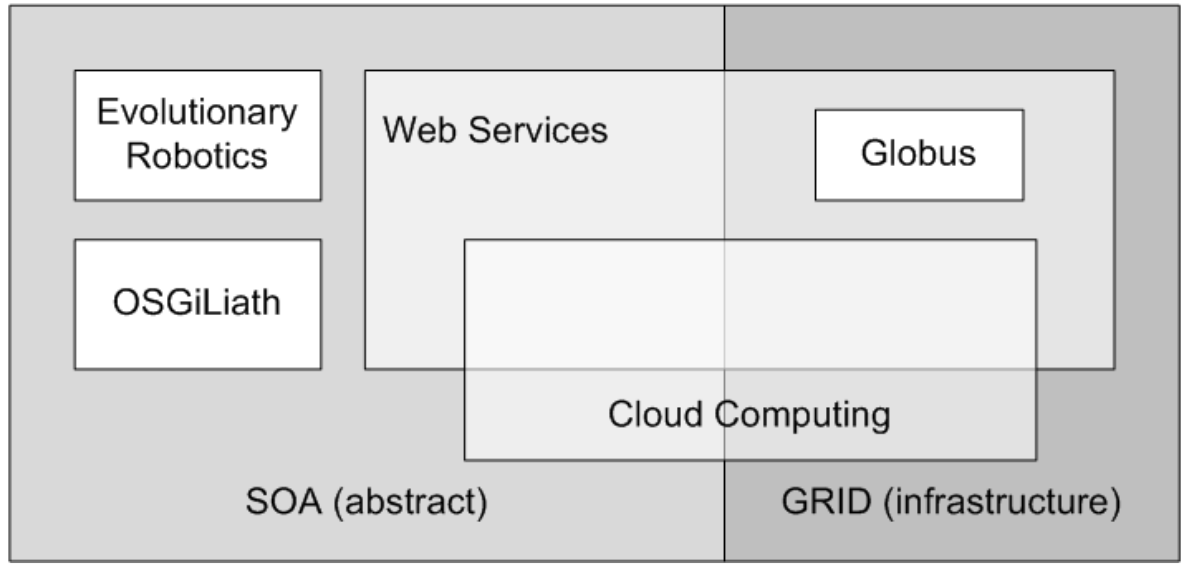
\includegraphics[width=26pc]{gfx/soa/soagrid.jpg}
\caption{SOA as abstract paradigm to develop in different EAs areas. Using specific technologies such as Web Services allows grid integration.}
\label{fig:soagrid}
\end{SCfigure}
We are going to use SOMA guidelines (identification, specification and realization of the services, flows and components) because is the methodology more flexible and less focused to commercial purposes. Next chapter will explain the design principles of SOA for developing services for EAs. Then, a specific SOA technology will be used to develop an implementation of a service oriented architecture for EAs.